\documentclass [11pt]{article}						
\usepackage{fancyhdr}
\usepackage[utf8]{inputenc}
\usepackage[english]{babel}
\usepackage{gensymb}
\usepackage{amsmath,amssymb,amsfonts}
\usepackage{algorithmic}
\usepackage{graphicx}
\usepackage{textcomp}
\usepackage{xcolor}
\usepackage{siunitx}
\usepackage{indentfirst}
\usepackage[margin=2.5cm]{geometry}
\usepackage{float}
\usepackage{hyperref}
\usepackage[UKenglish]{datetime}
\usepackage{setspace}
\usepackage{hhline}

\hypersetup
{
    colorlinks=true,
    linkcolor=black,   
    urlcolor=blue,
}

\pagestyle{fancyplain}
\fancyhf{}
\fancyhead[R]{Student No. 10618407}
\fancyfoot[R]{\thepage}

\doublespacing

\begin{document}							
\title{\bf AINT351Z - Learning, Planning, and Control of a Planar Arm Coursework 2021} 	
\author{Student No. 10618407} 								
\date{\today} 										
\maketitle 												
\pagenumbering{roman}			
\newpage			
\setcounter{page}{2}								
\tableofcontents 
\newpage

\section{Training Data Generation}	
\subsection{Display workspace of the Revolute Arm}
\pagenumbering{arabic}

The code in figure~\ref{fig:codeForArm} intialises the arm that is used. It plots an arm with length L1, and L2 which are shown below. The two joint angles are generated using the 'generateUniformDistribution' shown in figure~\ref{fig:uniformDistribution}.

\begin{figure}[H]
\centerline{\includegraphics[width=12cm]{generateArmDataCode}}
\caption{Code for generating the 2DOF arm}
\label{fig:codeForArm}
\end{figure}

These angles are between zero and pi, and are used in the provided ‘RevoluteForwardKinematics2D’ function. This is used to calculate and return the location of the arm’s elbow and end effector, point1 and point 2 respectively. This can be seen in figure~\ref{fig:codeForArm}.

\begin{figure}[H]
\centerline{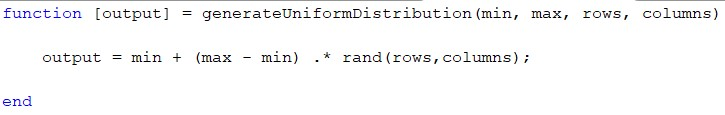
\includegraphics[width=12cm]{generateUniformDistribution.jpg}}
\caption{Generate Uniform Distribution Code}
\label{fig:uniformDistribution}
\end{figure}

Once the data for the arm is generated, the useful range of this arm was outputted using the code in figure~\ref{fig:codeToPlotWorkspace}. The output plot is shown in figure~\ref{fig:outputtedWorkSpace}.

\begin{figure}[H]
\centerline{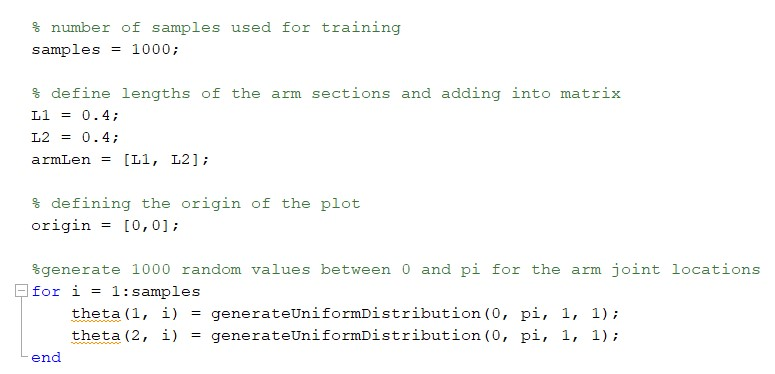
\includegraphics[width=12cm]{GenerateArmDataCode}}
\caption{Code to plot the workspace of the 2DOF arm}
\label{fig:codeToPlotWorkspace}
\end{figure}

\begin{figure}[H]
\centerline{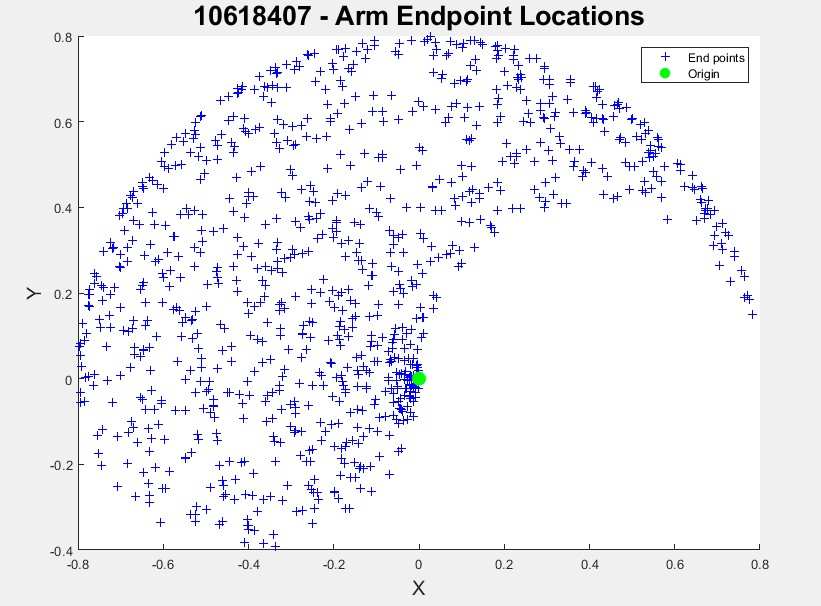
\includegraphics[width=9cm]{arm_endpoint}}
\caption{Output workspace of the 2DOF arm}
\label{fig:outputtedWorkSpace}
\end{figure}

Figure~\ref{fig:outputtedWorkSpace} shows the useful range, also known as the workspace, of the arm. This shows all the points that the end effector can reach. This arm is a 2DOF arm with endpoints highlighted with blue crosses and an origin highlighted by a green dot (at 0,0). This workspace is known as a tear-drop swirl pattern. The length from the end point to the origin is 0.8m. With the shoulder joint (origin of the robot), and the elbow joint being limited to range between zero and pi, the possible locations of the end effector are restricted. The shape of the resulting workspace would dictate the possible applications for the robot. It is important to keep this in mind for potential applications. The size of this workspace (approximately $5.8m^2$), will be important when deciding appropriate final scaling of the maze in later tasks. 

\section{Implement 2-layer network}
\subsection{Implement 2-layer network training}

\begin{figure}[H]
\centerline{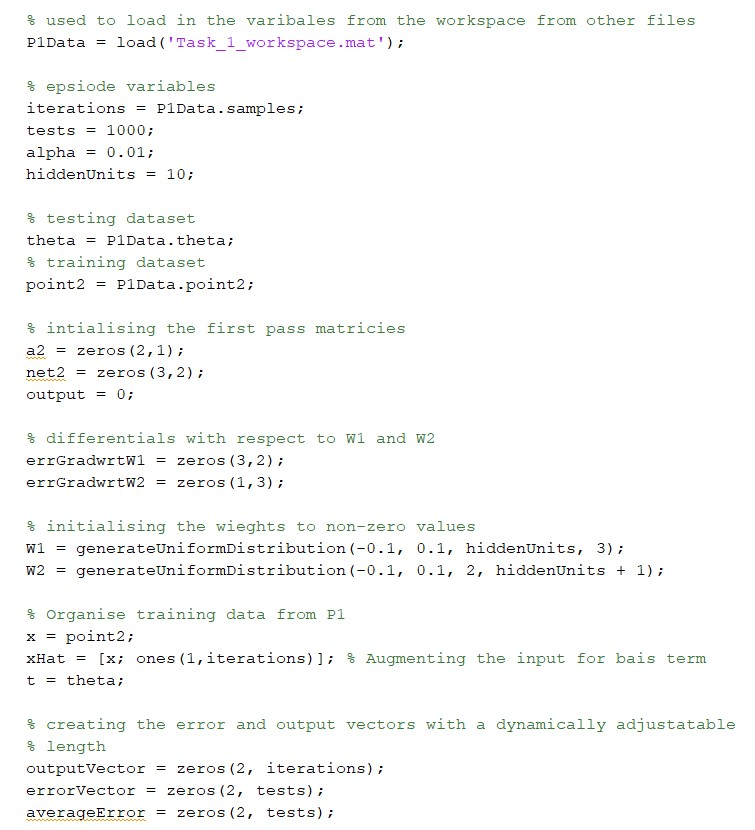
\includegraphics[width=12cm]{Neural_network_defintions}}
\caption{Setting up and importing constants and variables used for training the network}
\label{fig:neuralNetworkDefinitions}
\end{figure}

The weights are initialised using the 'generateUniformDistribution' function shown in figure~\ref{fig:uniformDistribution}. The values are initialised to be between -0.1 and 0.1. $W1$ is set up as a $'hiddenUnits'$ x $3$ matrix , and $W2$ is a $2$ x $'hiddenUnits+1'$ matrix. The $'hiddenUnits'$ variable has been used so that the values can be adjusted easily to test different configurations. It is important for the weights to be close, but not equal to, zero. This would cause symmetry in the model which would mean all the inputs to the nodes are also zero. This would mean that no data is being transferred through any of the zero nodes. 

\begin{figure}[H]
\centerline{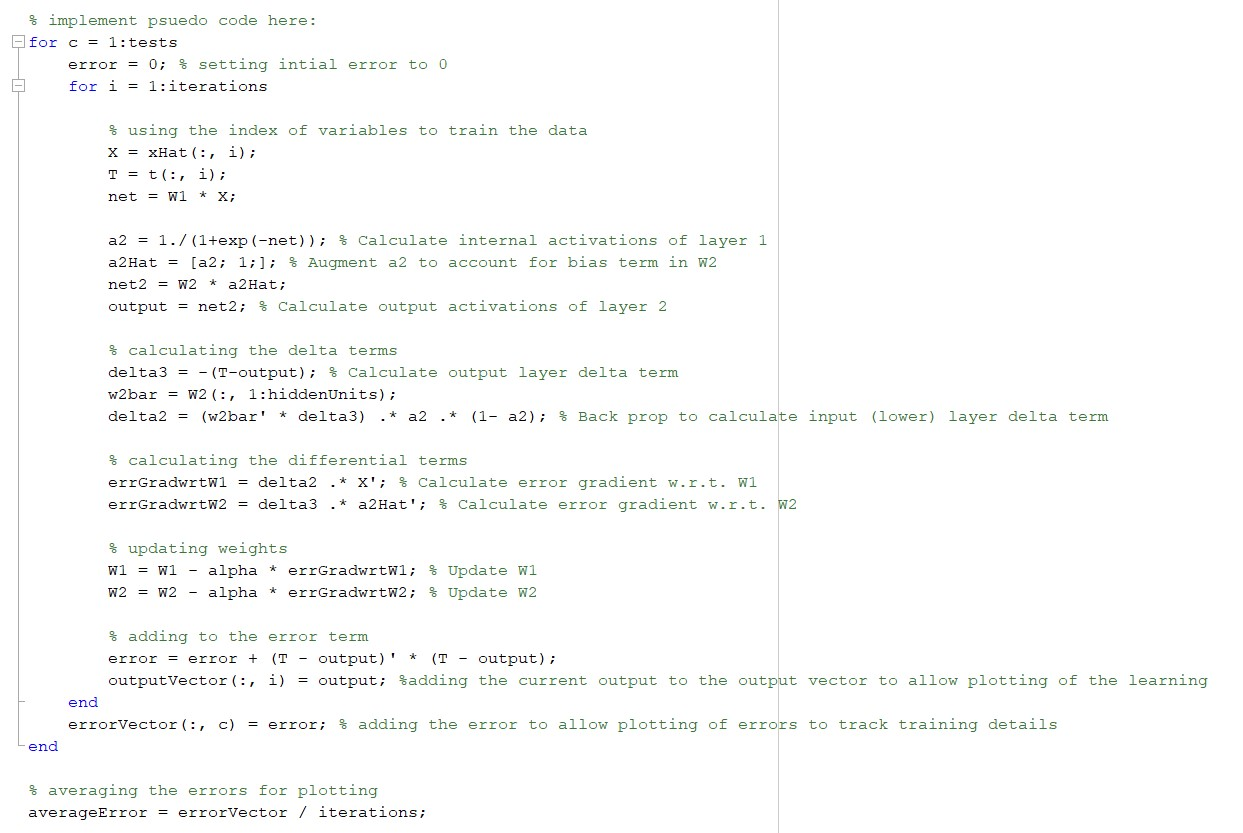
\includegraphics[width=15cm]{Neural_network_training}}
\caption{2-layer network with 10 hidden units and a linear output}
\label{fig:2-layer_network}
\end{figure}

The figure above shows a neural network that works by defining the weights of the layers, using given training and target samples. The network calculates and recalculates the weights as many times as is defined by the 'tests' variable. In this instance, tests is 1000. After this, the values are used to calculate the internal and output activation layers of the network.  The internal activation values are used to train the weight values using back propagation. The output error term is calculated by evaluating the difference between the actual output of the network and the output predicated by the target value of the network. The gradient of the weights is calculated by multiplying the input and output activations by the input values. This gradient is multiplied by the learning rate, alpha, and is taken away from the weights. This is used to refine the values of the weights. These weights are used as the new weights for the next pass of the network. The error term for all the samples for both W1 and W2 is calculated from the learning pass. This can be plotted to see the progress of the network throughout it's learning passes. This can be seen in figure~\ref{fig:errorOverIterations} below.


\subsection{Train network inverse kinematics}

The training of the Inverse Kinematics was implemented using a feedforward pass that is shown in the code below. 

\begin{figure}[H]
\centerline{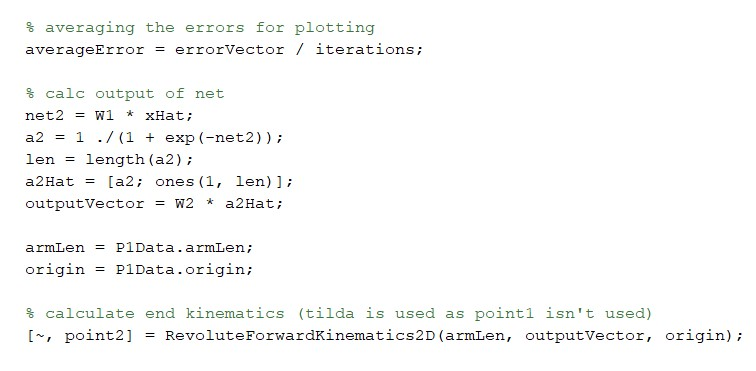
\includegraphics[width=12cm]{Neural_network_feed_forward}}
\caption{Feedforward pass of the Network}
\label{fig:feed_forward_pass}
\end{figure}

The corresponding error over the number of iterations, and the output work space of the arm trained using the network, can be seen below in figure~\ref{fig:errorOverIterations} and figure~\ref{fig:Training Workspace of the endpoint of a 2 link arm before and after training} respectively.

\begin{figure}[H]
\centerline{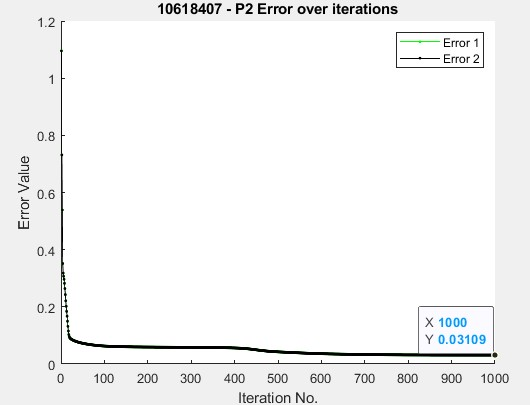
\includegraphics[width=12cm]{error_over_itterations}}
\caption{Error over iterations throughout network learning and feedforward pass}
\label{fig:errorOverIterations}
\end{figure}

It can be seen from the diagram that at 1000 tests, the output error has dropped to 0.03109. This has been evaluated against other configurations ie. different number of tests and hidden layers. These results are outlined below. 

\subsection{Test and improve the inverse model}

\begin{figure}[H]
\centerline{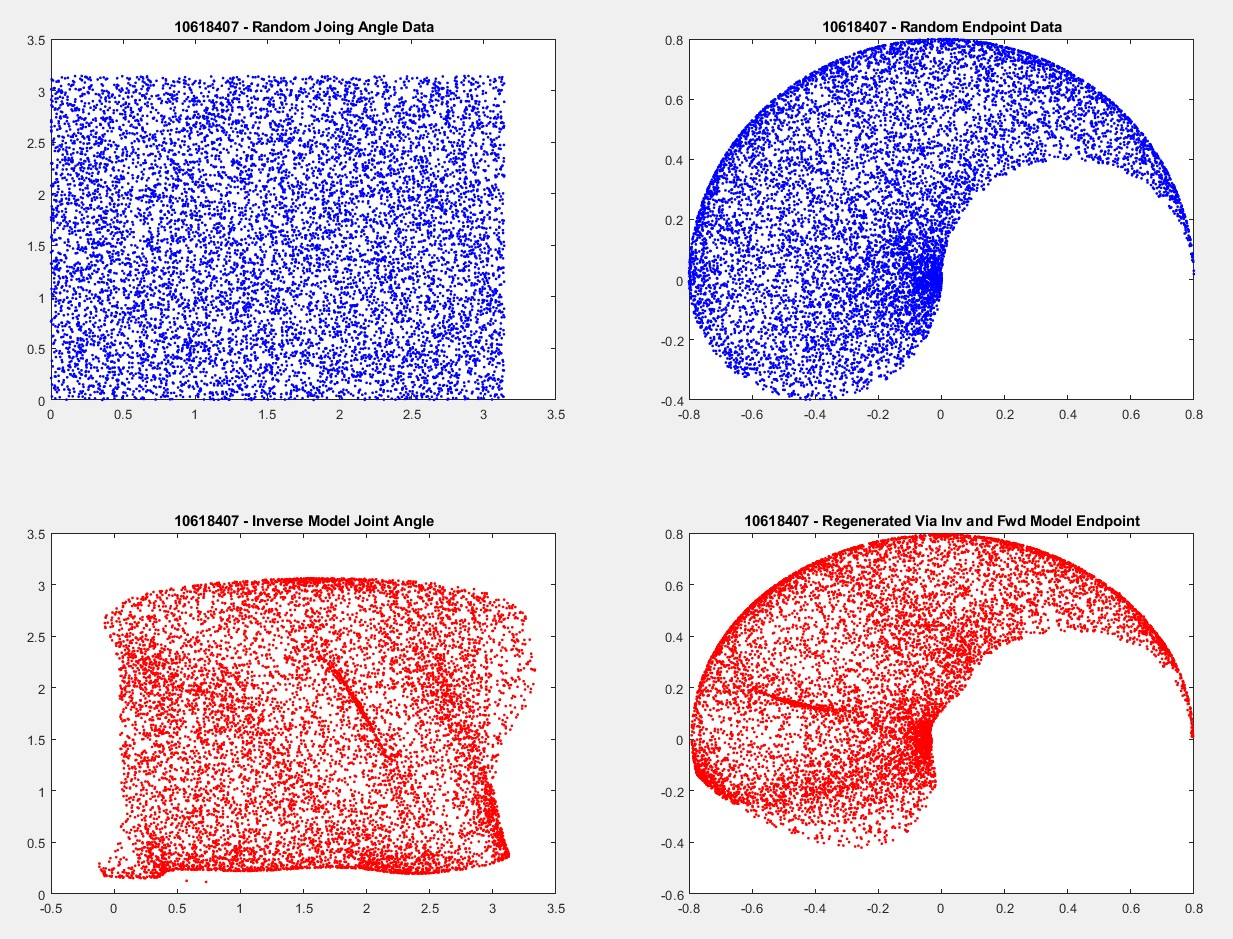
\includegraphics[width=15cm]{training_workspace_of_the_endpoint-of_a_2-link_arm}}
\caption{Training workspace of the endpoint of a 2 link arm before and after training}
\label{fig:Training Workspace of the endpoint of a 2 link arm before and after training}
\end{figure}

In figure~\ref{fig:Training Workspace of the endpoint of a 2 link arm before and after training}, the top set of plots show the attainable locations of the arm along with the angles of each of the points used to get to those locations before the network was trained. The bottom set of these plots show the same data but after the network was trained. \\
This figure is significant because it shows the overall shape of the robot's workspace has been mostly preserved from the random angles initially used. There are however, some differences in the plot of the arm, primarily between $[0, -0.2]$ and $[0, 0.2]$. This could be for several reasons. I believe that it is primarily because of the size of the data set being used to train the model. Ideally, the model would be trained with a much larger data set which would give a more comprehensive set of data to train the model. This could alleviate those areas which contained gaps in the model. 

To make a more comprehensive dataset for training the arm, we need to increase the number of angle samples. To increase the usefulness of the task, and to make the dataset more representative, it would be useful to be able to create more samples inside the larger end of the teardrop. This is where most of the arm's movement will take place. This would create finer granularity in the areas of the robot's workspace that would be most often utilised. This could lead to increased accuracy in the robot's movements within the maze. The data set could be further increased by using more representative data from 'accurate' paths through the maze. This would allow the robot to be able to train of data that is actually representative of the task it would be performing. The majority of the network learning has been genetic pre training of the arm. This allows it to plot joint angles to a given endpoint of the arm. It would but useful to train the arm on more maze solving data. This would allow it to become more effective in performing that specific task. This could allow the arm to perform better when attempting to solve the maze.

The figures below show the output of the neural network with different values for the number of tests run, alpha (learning rate), and the number of hidden nodes. 

\begin{figure}[H]
\centerline{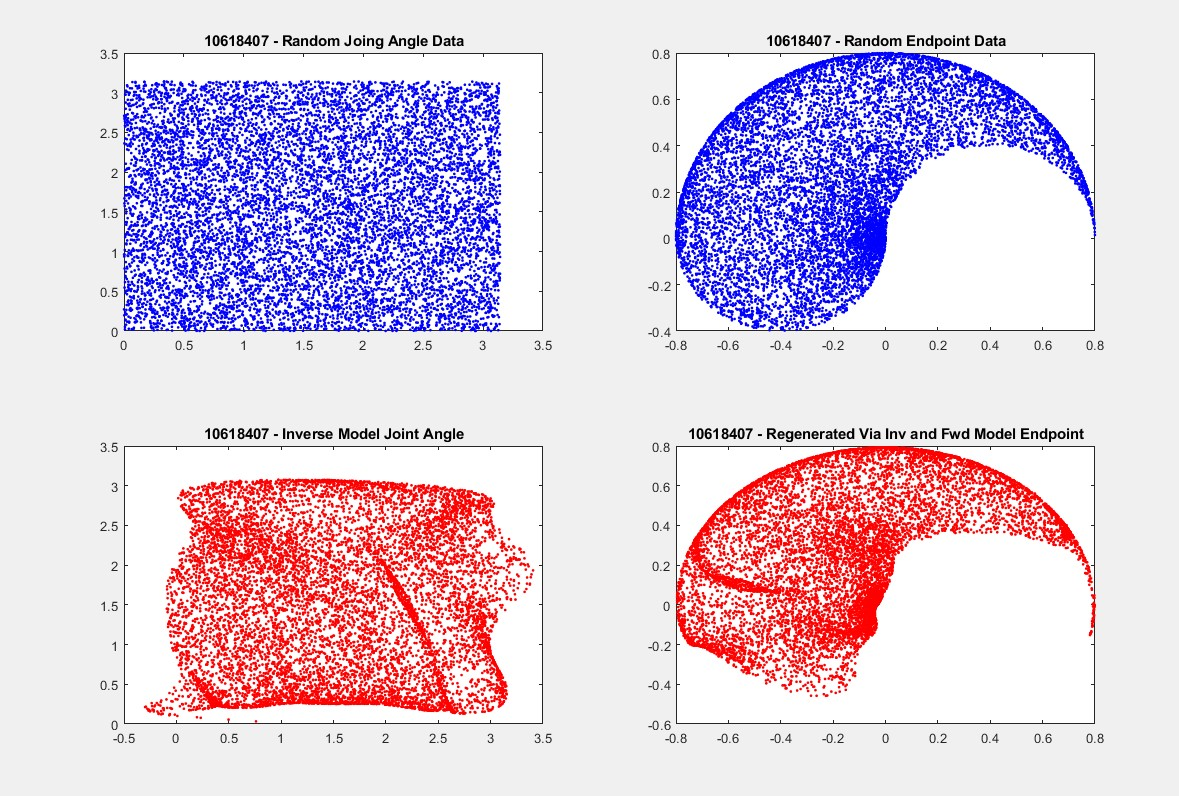
\includegraphics[width=15cm]{training_workspace_of_the_endpoint-of_a_2-link_arm_100_hidden_layers}}
\caption{Training Workspace of the endpoint of a 2 link arm before and after training No. of hidden nodes changed from 10 to 100}
\label{fig:nodes_10to_100}
\end{figure}

As seen in figure~\ref{fig:nodes_10to_100}, increasing the number of hidden nodes from 10 to 100 has a detrimental effect on the training of the robot's workspace. The disparity between the two can be seen mainly in the bottom of the larger end of the teardrop. It has lost the curved shape of the teardrop which negatively impacts on the size of the arm’s workspace.

\begin{figure}[H]
\centerline{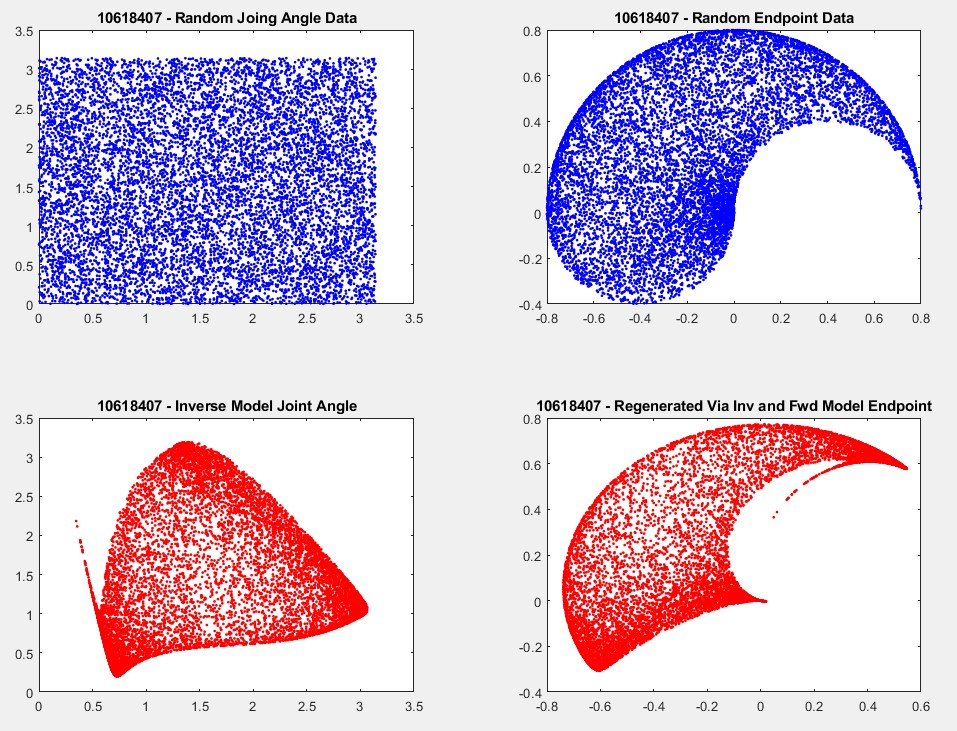
\includegraphics[width=15cm]{training_workspace_of_the_endpoint-of_a_2-link_arm_2_hidden_layers}}
\caption{Training Workspace of the endpoint of a 2 link arm before and after training No. of hidden nodes changed from 10 to 2}
\label{fig:nodes_10to_2}
\end{figure}

As seen in figure~\ref{fig:nodes_10to_2}, decreasing the number of hidden nodes from 10 to 2 also has a detrimental effect on the training of the robot arm. Unlike increasing the number of hidden nodes, the disparity between the two plot is far more pronounced. Although there are a few remenents of the previous teardrop shape, it is significantly warped and the workspace is drastically changed. The overall size of the robot's workspace decreased, making it less effective.

\begin{figure}[H]
\centerline{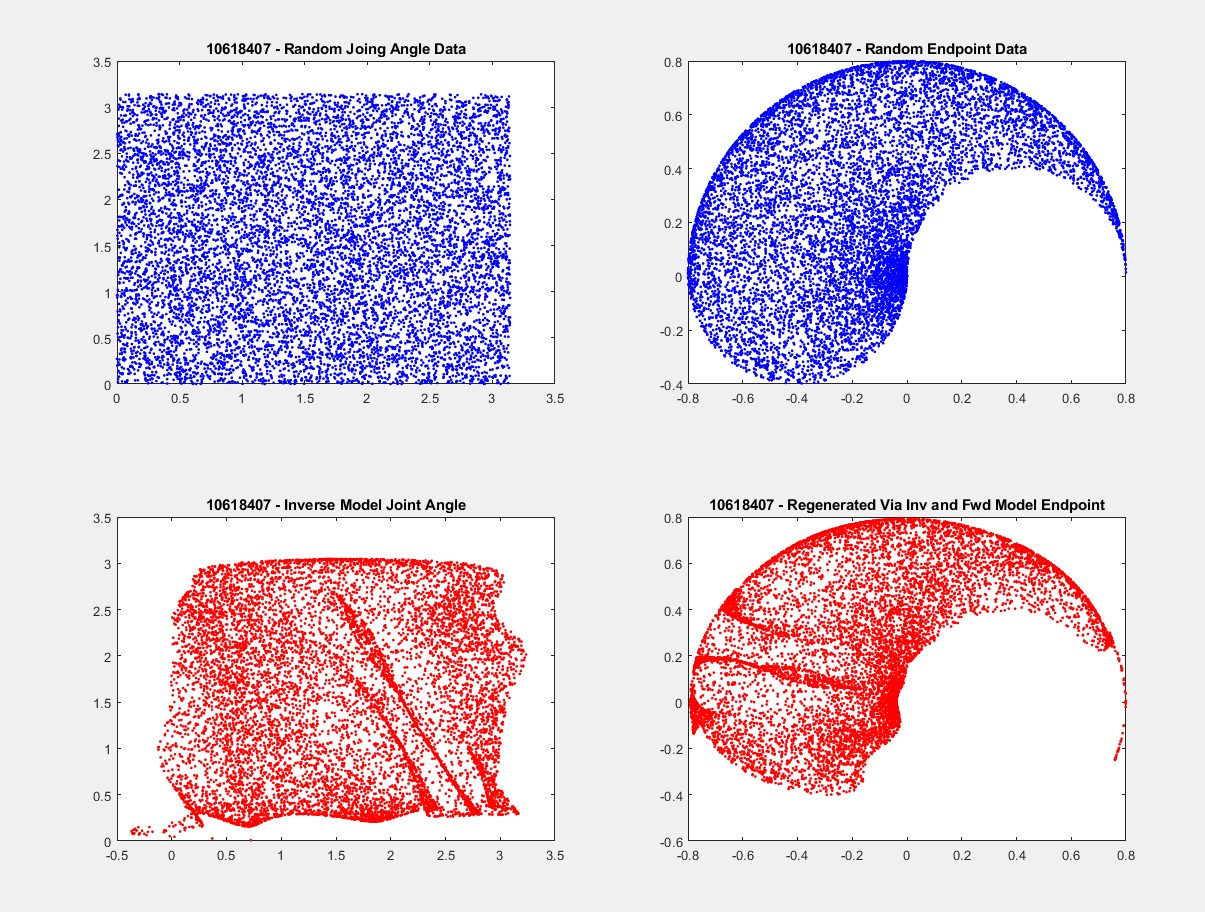
\includegraphics[width=15cm]{training_workspace_of_the_endpoint-of_a_2-link_arm_10000_tests}}
\caption{Training Workspace of the endpoint of a 2 link arm before and after training No. of tests changed to 10000}
\label{fig:test_1000_to_10000}
\end{figure}

As shown in figure~\ref{fig:test_1000_to_10000}, increasing the number of tests leads to a very similar model shown with only 1000 tests, with mostly the same shape as the initial training. Although the area has been more thoroughly tested, there are some invalid results in the bottom left hand of the Inverse Model Joint Angle plot. This could be because the model was overtrained by using too many tests. Despite this, the overall output shape remains consistent to the origin. It takes far longer to train the network on each iteration and the output can be seen as invalid. 

\begin{figure}[H]
\centerline{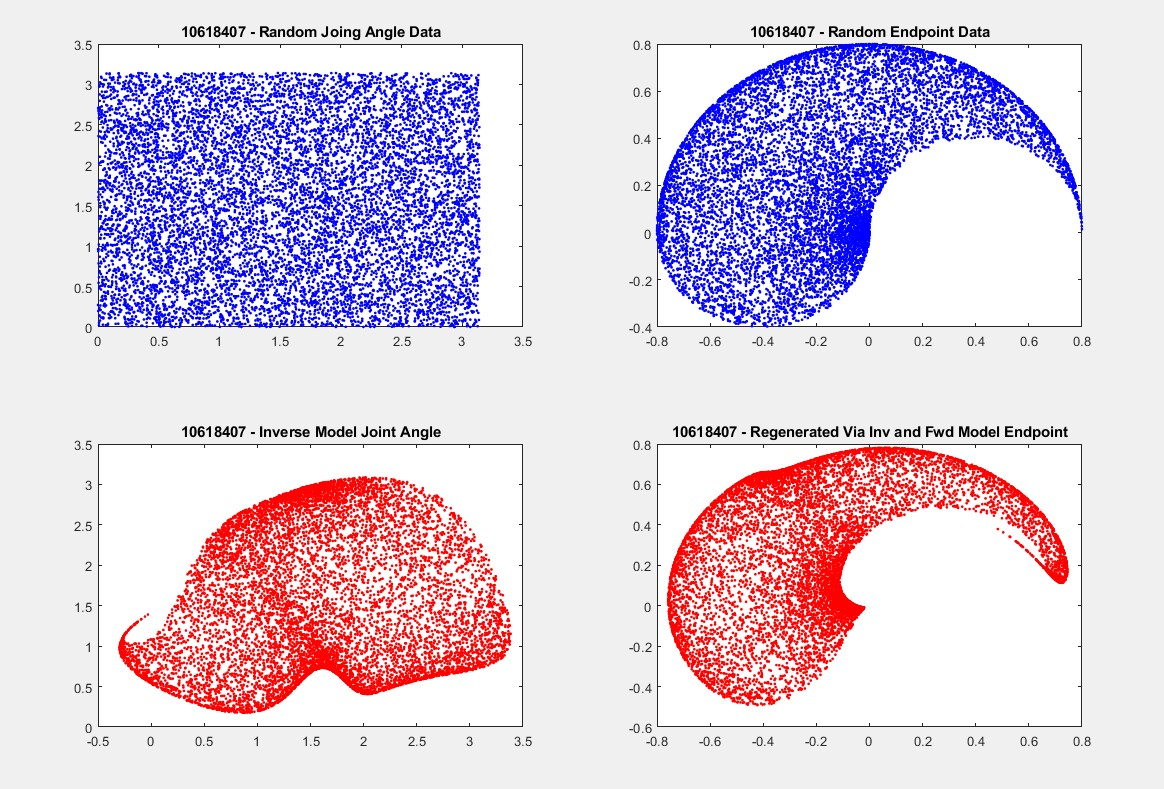
\includegraphics[width=15cm]{training_workspace_of_the_endpoint-of_a_2-link_arm_alpha_0001}}
\caption{Training Workspace of the endpoint of a 2 link arm before and after training - Alpha changed to 0.0001}
\label{fig:alpha_0.0001}
\end{figure}

\begin{figure}[H]
\centerline{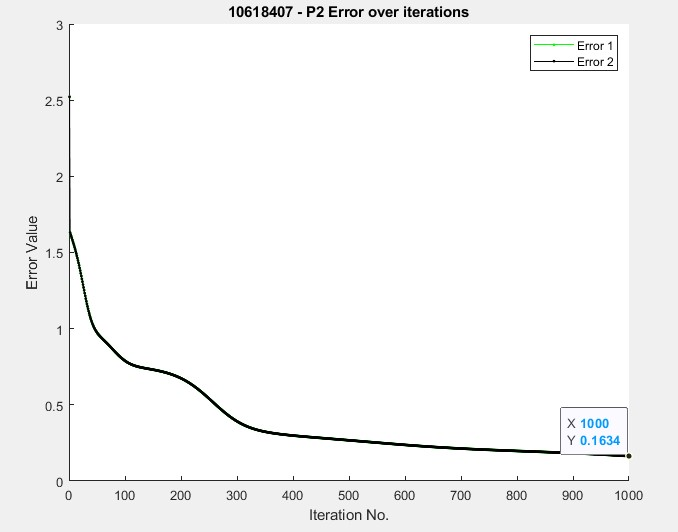
\includegraphics[width=10cm]{error_over_itterations_alpha_0001}}
\caption{Error over iterations throughout network learning and feedforward pass - Alpha changed to 0.0001}
\label{fig:error_alpha_0.0001}
\end{figure}

As seen in figure~\ref{fig:alpha_0.0001} and figure~\ref{fig:error_alpha_0.0001}, the values of alpha have a very large effect on the neural network. Not only is the workspace effected, but so is the error. The workspace is significantly less comparable to the original, it is more comparable to the workspace with only two hidden nodes. Whilst still retaining the original teardrop shape, it has been severely deformed around the top and at the thin end. It can also be seen, much like the workspace of the training with 10000 tests, there are some angles that the arm cannot achieve, outlined in the bottom left hand side of the Inverse Model Joint Angle diagram. This is undesirable as it is training the model with unattainable angles. The ending error can also be seen to be considerably larger than in figure~\ref{fig:errorOverIterations}. The error resulting from an alpha rate of 0.0001 is over five times larger than the original error.
  
\section{Path through a maze}
\subsection{Random start state}

\begin{figure}[H]
\centerline{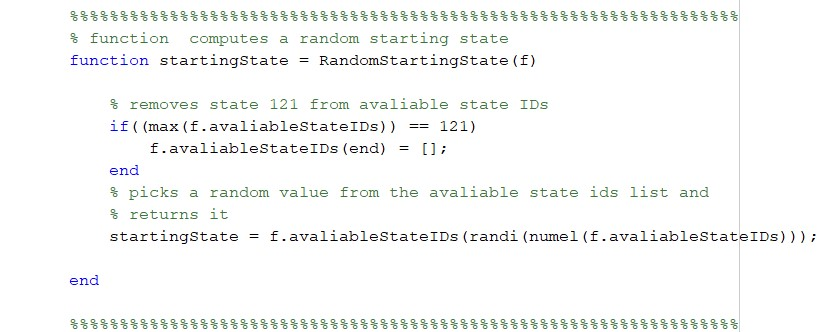
\includegraphics[width=15cm]{random_starting_state}}
\caption{Random starting state selected from ‘avaliableStateIDs’ (creation of ‘avaliableStateIDs’ is shown below)}
\label{fig:rand_starting_state}
\end{figure}

\begin{figure}[H]
\centerline{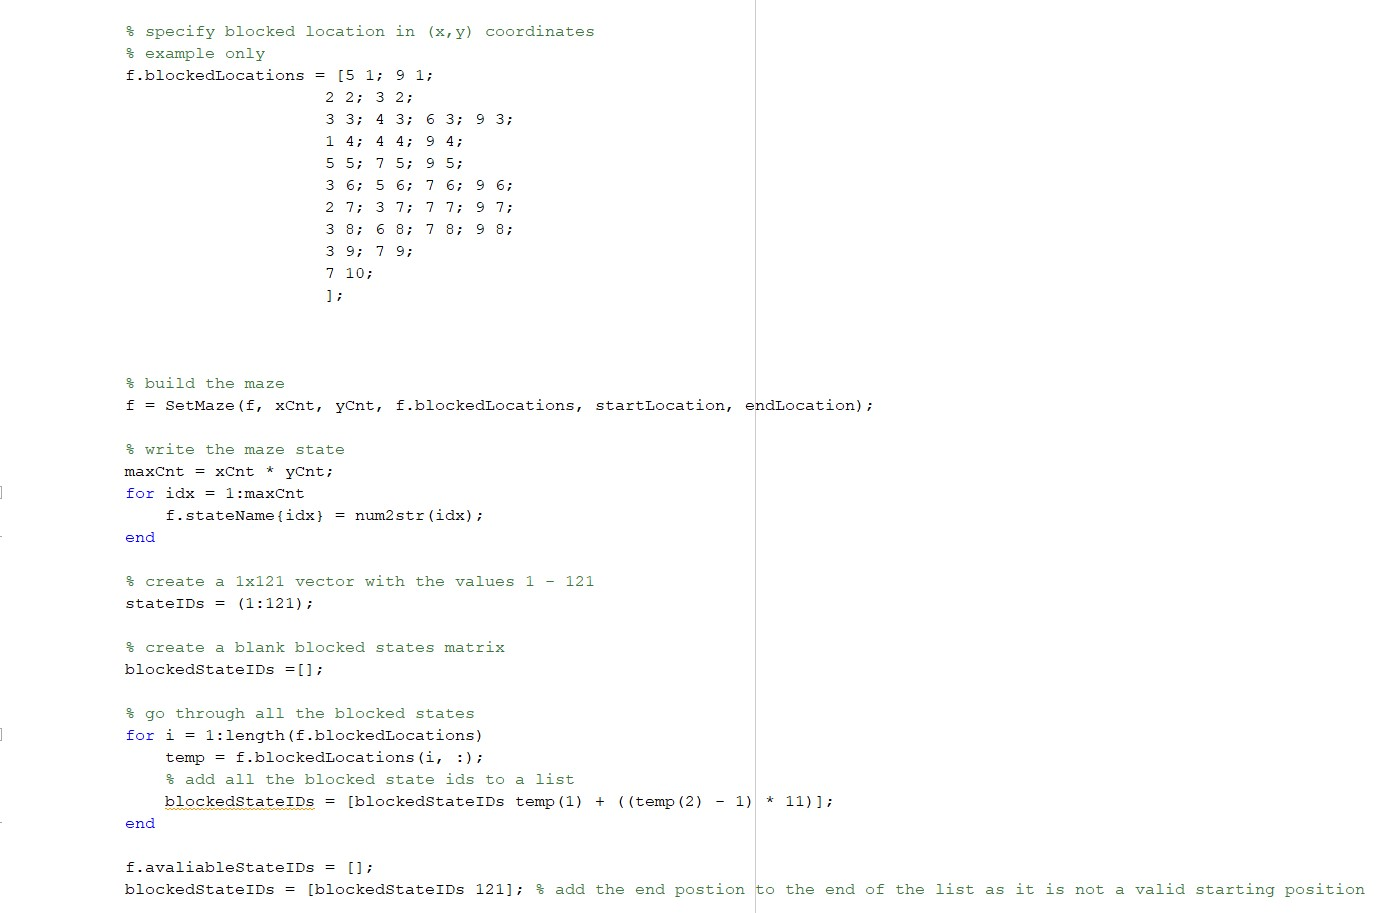
\includegraphics[width=15cm]{blocked_states}}
\caption{Code to create blocked ids and ‘blockedStateIDs’}
\label{fig:blocked_state_and_blocked_state_ids}
\end{figure}

\begin{figure}[H]
\centerline{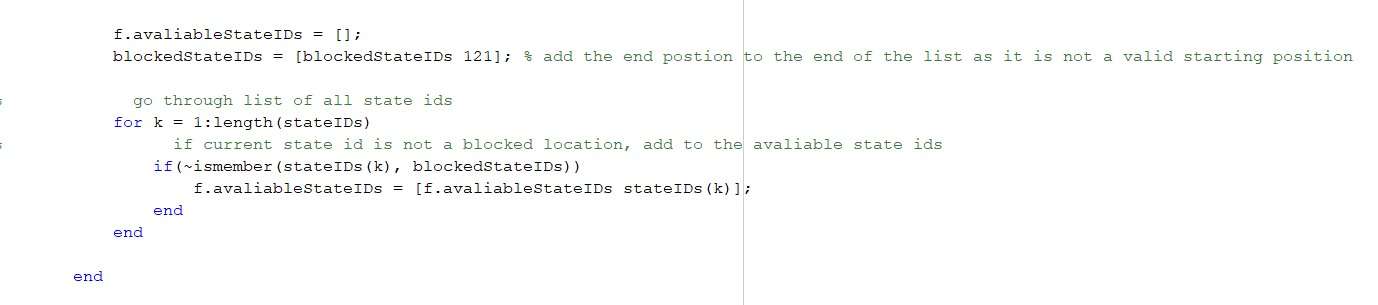
\includegraphics[width=15cm]{blocked_states_and_avaliable_states}}
\caption{Code to create ‘avaliableStateIDs’ }
\label{fig:avaliable_state_ids}
\end{figure}

As shown in the figures above, blocked state IDs are found by adding all the blocked IDs in coordinate form to a big list. The valid state IDs are found by creating a list from 1-121 and any state IDs that are also in the blocked IDs list get removed. This leaves you with just the available state ids which are used to calculate the valid random starting state IDs, amongst other things that are outlined later. 

\begin{figure}[H]
\centerline{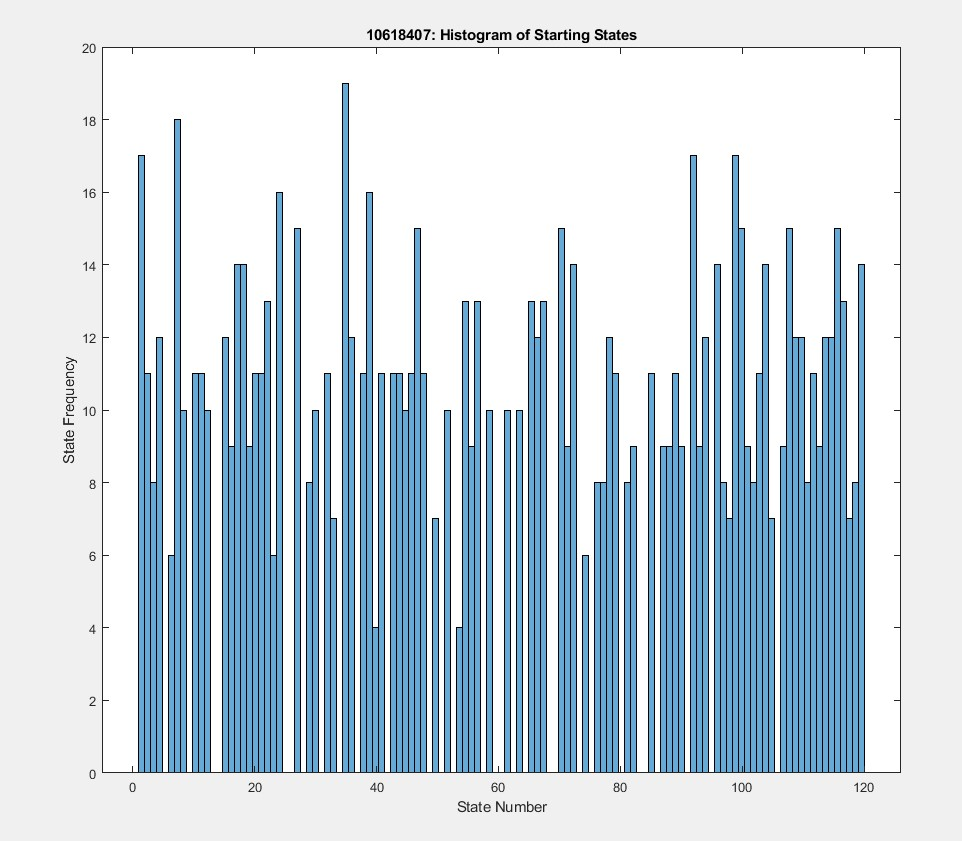
\includegraphics[width=15cm]{Histogram_of_starting_states}}
\caption{Histogram of 1000 generated starting state ids}
\label{fig:random_state_ids_histogram}
\end{figure}

The histogram in figure~\ref{fig:random_state_ids_histogram} shows 1000 randomly generated values for the maze. Each of the bins in the maze correspond to a state ID. There are gaps throughout the histogram. These gaps coincide with blocked or invalid starting state IDs. The values 1 and 121 are also blank as these are not valid starting IDs for the random starting state selector. The distribution of these values is not uniform, but as the number of random starting state ids increases, the distribution would tend towards a more uniform distribution. 

The code to display this histogram is shown below.

\begin{figure}[H]
\centerline{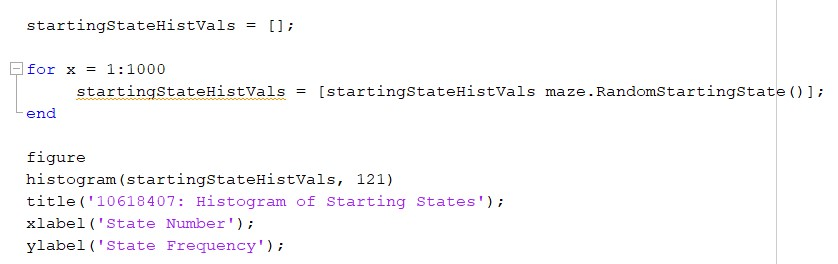
\includegraphics[width=15cm]{code_to_output_start_state_histo}}
\caption{Code to generate the starting state histogram}
\label{fig:random_state_ids_histogram_code}
\end{figure}

\subsection{Build a reward function}

\begin{figure}[H]
\centerline{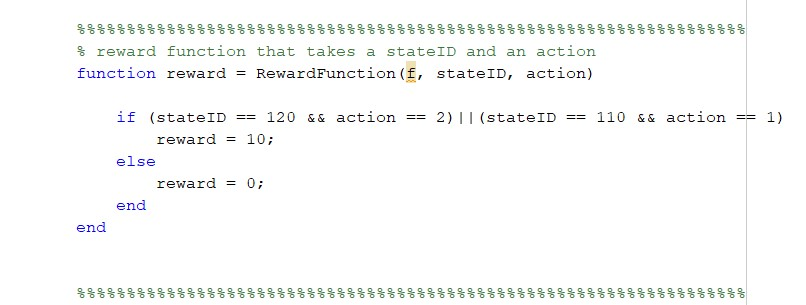
\includegraphics[width=15cm]{reward_function}}
\caption{Reward function that evaluates current state and proposed action to allocate reward}
\label{fig:reward_function}
\end{figure}

The reward function is implemented as part of the update Q-Value calculations. The reward is only given if the current state and proposed action leads to the goal state. In that case, the reward is 10. If these conditions are not met, the reward stays at zero. The states and actions to get a reward can be seen in figure~\ref{fig:reward_function} and this function can be changed to give a different end state reward. Although not utilised in this setup, it is possible to allocate a small negative reward for each move that is not a rewarding move. This can also be used to train the network. 

\subsection{Generate the transition matrix}

\begin{figure}[H]
\centerline{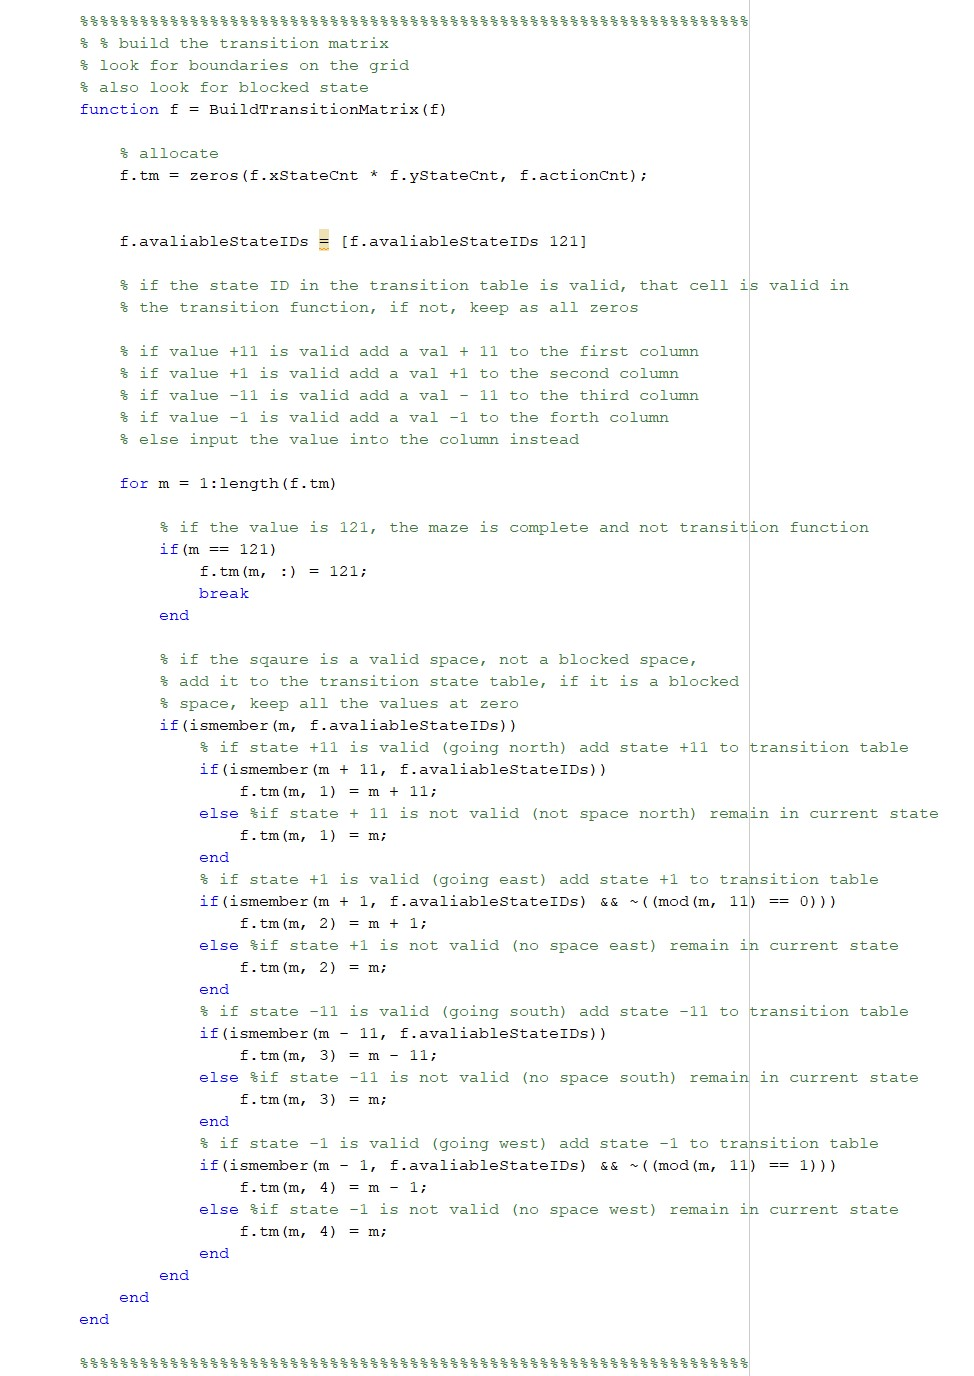
\includegraphics[width=12cm]{Transition_table}}
\caption{Function to build the transition matrix from the size of the maze and the available state ids}
\label{fig:tm}
\end{figure}

The transition matrix (tm) is built in the function above. It starts by adding 121 to the available state IDs list as for the tm, it is a valid state. It then iterates through the length of the empty tm and looks at the current value. If the value is 121, all the values in the tm go back to 121, as it cannot move out that state. The second check is to ascertain if the current ID of the tm is a member of the available state IDs. If the value isn’t a valid state, then do nothing (the values all stay equal to zero). If the state is an available state id, then the function checks if it can move north, east, south, or west and updates the tm as appropriate. If one or more of the north, east, south, or west moves cannot be achieved, the tm puts back in the value of the state id for the relative movement. This can be seen with the comments in the tm function code. This is done for all values in the tm.

\subsection{Initialize Q-values}

\begin{figure}[H]
\centerline{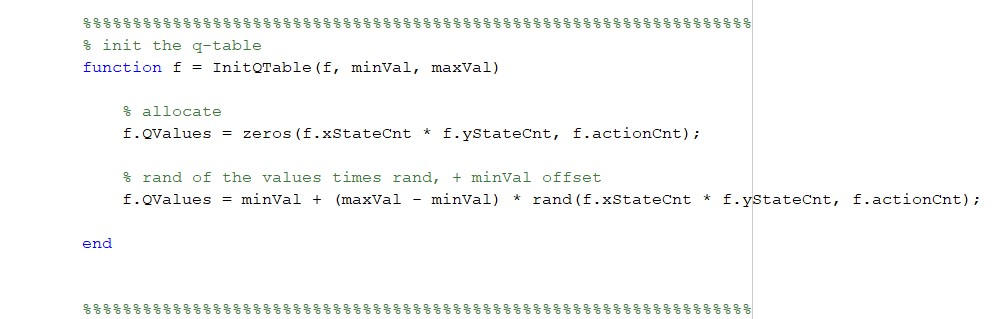
\includegraphics[width=15cm]{initialise_q_values}}
\caption{Function to initialise the Q-Values}
\label{fig:init_q_vals}
\end{figure}

\begin{figure}[H]
\centerline{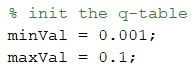
\includegraphics[width=5cm]{init_q_values_values}}
\caption{Q-Table initialisation values }
\label{fig:init_q_val_vlaues}
\end{figure}

The ‘InitQTable’ function starts by creating a matrix of all zeros, which is the size of the maze (11x11). Values are then randomly created between the ‘minVal’ and ‘maxVal’ seen in the figure above. These values are put in a matrix that is the size of the maze and overwrites the QValues table of all zeros. 

\subsection{Implement DynaQ-learning algorithm}

\begin{figure}[H]
\centerline{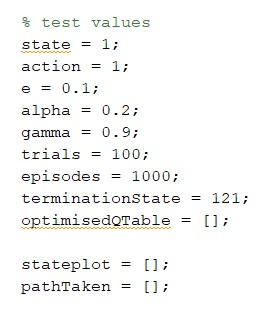
\includegraphics[width=5cm]{Q-learning_values}}
\caption{Initialisation of variables for the Q-Learning}
\label{fig:init_values_for_q_learning}
\end{figure}

\begin{figure}[H]
\centerline{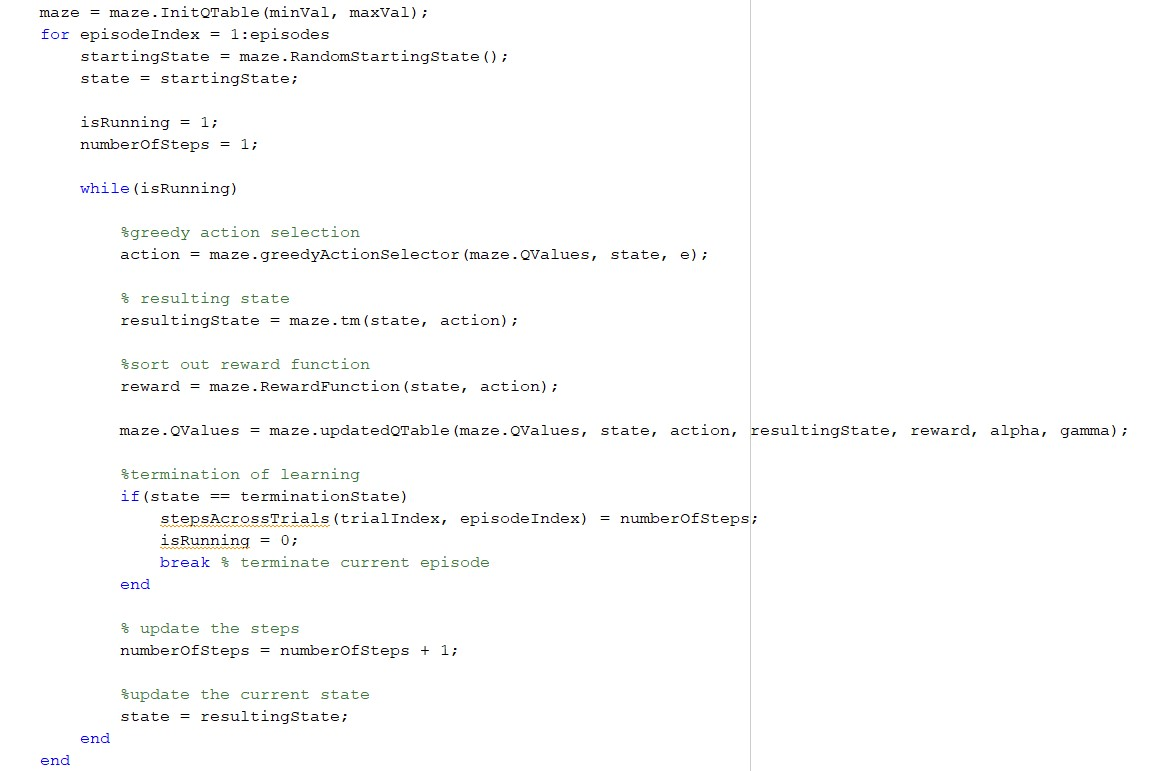
\includegraphics[width=15cm]{Q-learning-implementation}}
\caption{Main Q-Learning Algorithm (runs in the main function)}
\label{fig:q-learing}
\end{figure}

The main Q-learning algorithm runs inside of the 'Main\_P3\_RunGridworld2021.m' file. The initial variables are setup as shown in figure~\ref{fig:q-learing} above. The purpose of this main algorithm is to update the Q-Values, which are based on a multitude of different variables. These include the $\varepsilon$-greedy function, outlined in figure~\ref{fig:e-greedy_function}, the reward function, the learning rate alpha, and gamma. The while loop keeps the Q-learning updating the Q-Values and traversing the maze until the goal state is reached. Once this occurs, the Q-learning will exit that loop and restart the learning from a new random starting state, with the updated Q-Values from the old run. This loop will continue until it has completed the full episode number of loops, continuing to optimise the Q-Values whilst solving the maze. 

\begin{figure}[H]
\centerline{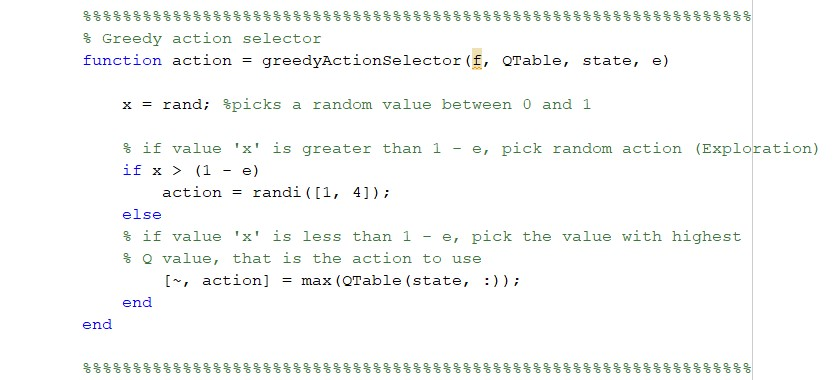
\includegraphics[width=15cm]{greedy_action}}
\caption{$\varepsilon$-greedy Action Selector}
\label{fig:e-greedy_function}
\end{figure}

The $\varepsilon$-greedy function chooses the next action given the current state. There are two possible options for which state the action selector can choose: the action with the highest Q-Value or a random action. This is decided by selecting a random number between zero and one. If the number is greater than one minus $\varepsilon$ the random action is chosen. If the number is less than one minus $\varepsilon$, then the action with the highest Q-Value is chosen. This is to allow for some random exploration for new or not fully optimised Q-Values. 

\begin{figure}[H]
\centerline{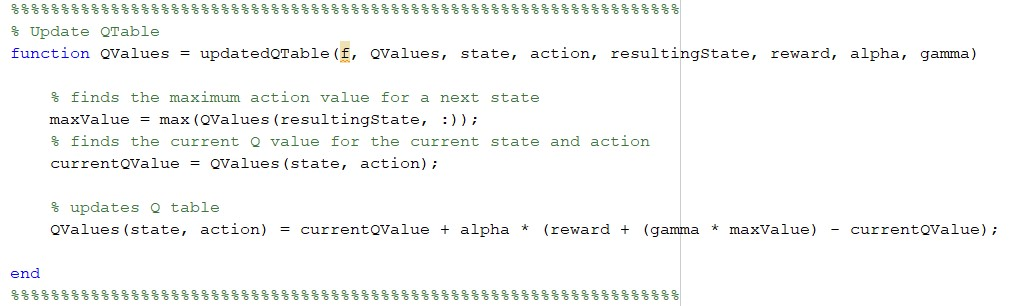
\includegraphics[width=15cm]{update_q-table}}
\caption{Update Q-Table function }
\label{fig:update_q_table}
\end{figure}

The Update Q-Table function is called to update the Q-Values in the Q-Table at the end of each loop. These Q-Values are saved and optimised between each episode, helping the algorithm to learn.

\subsection{Run DynaQ-learning}

\begin{figure}[H]
\centerline{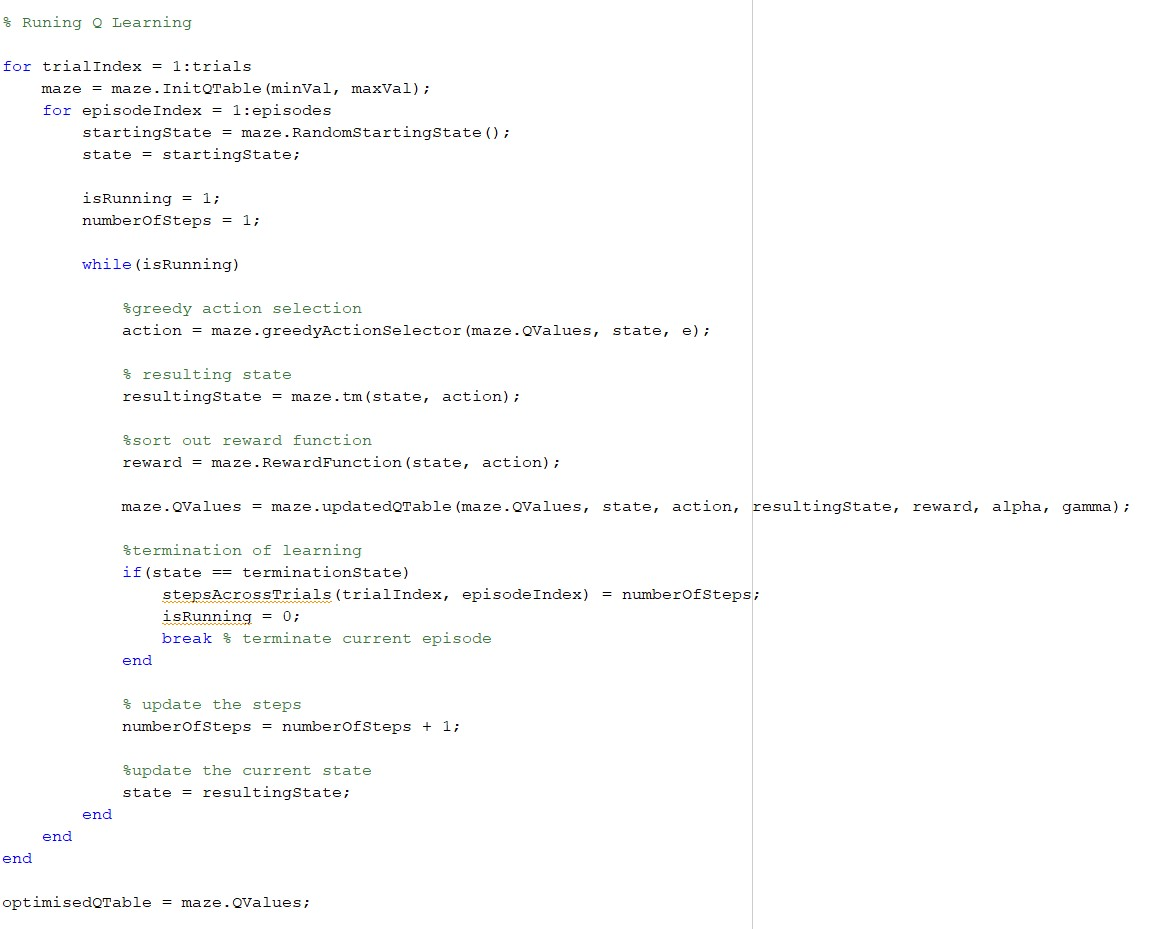
\includegraphics[width=15cm]{Q-learning_trials}}
\caption{Trial loops for Q-learning episodes}
\label{fig:q_learning_trials}
\end{figure}

A Q-learning trial is where the Q-Table is renewed with a freshly initialised Q-Table. The algorithm is then run again. This allows us to visualise when the program reaches the end state in the minimal number of steps. This could lead to a reduction of needed episodes and constant changes to reach the end state. 

\begin{figure}[H]
\centerline{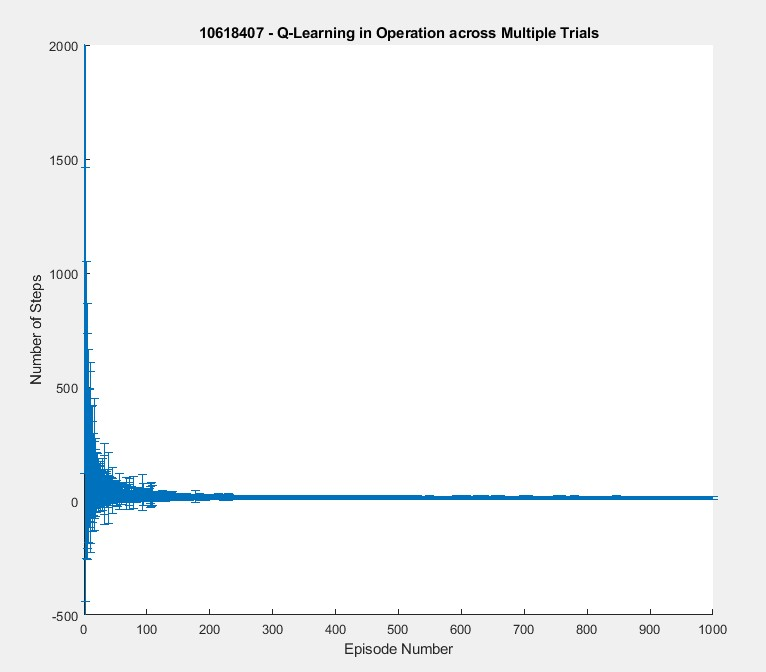
\includegraphics[width=15cm]{Q-learning_in_operation_across_multiple_trials}}
\caption{Error plots of mean and standard deviation of the Q-learning over multiple trials}
\label{fig:error_plot_across_multiple_trials}
\end{figure}

Figure~\ref{fig:error_plot_across_multiple_trials} above shows the error plots of the mean and standard deviation of the steps taken by the Q-Learning algorithm against the Episode Number. From Episode 250 onwards, the number of steps seems to remain consistent. This shows that the Q-Learning algorithm has likely found the most efficient way to get to the end state from any starting state. 

\subsection{Exploitation of Q-values}

\begin{figure}[H]
\centerline{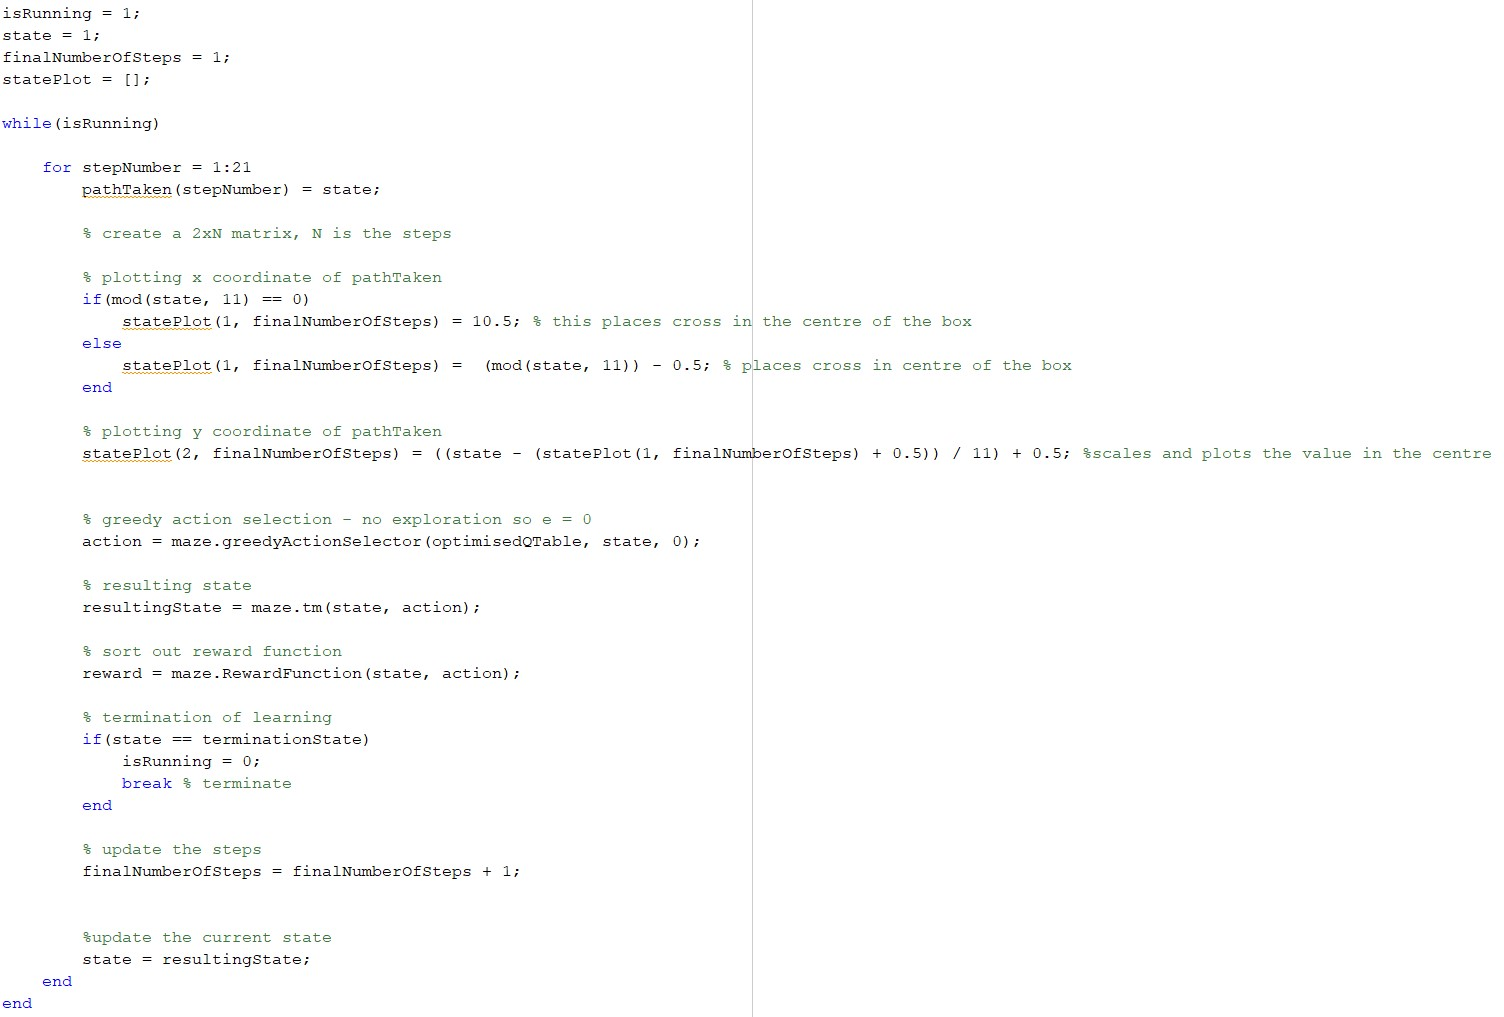
\includegraphics[width=15cm]{q-learning_with_exploration_set_to_zero}}
\caption{Running Q-Learning with epsilon set to zero}
\label{fig:q_learning_with_e_set_to_zero}
\end{figure}

This function is almost identical to the previous run through of the Q-Learning Algorithm except for two key differences. The first difference is that the epsilon value for the $\varepsilon$-greedy action selector is set to zero. This means that only the Q-Values are used to reach the end state (no exploration is done). The other key difference is that the Q-Table and values are not updated at each run through of the algorithm. This means that the Q-learning alogirthm has found the most optimised route to take through the maze. Three examples of optimal roots are shown in figure~\ref{fig:maze_solution_1}, figure~\ref{fig:maze_solution_2}, and figure~\ref{fig:maze_solution_3}.

\begin{figure}[H]
\centerline{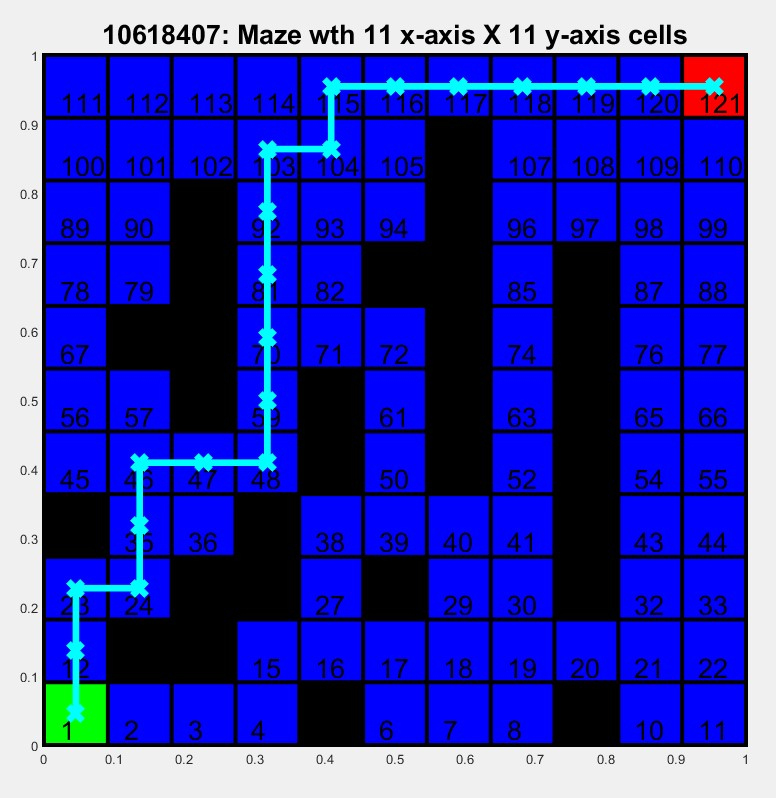
\includegraphics[width=9cm]{maze_solution_1}}
\caption{Plot of maze with path from highest Q-Values - solution 1}
\label{fig:maze_solution_1}
\end{figure}

\begin{figure}[H]
\centerline{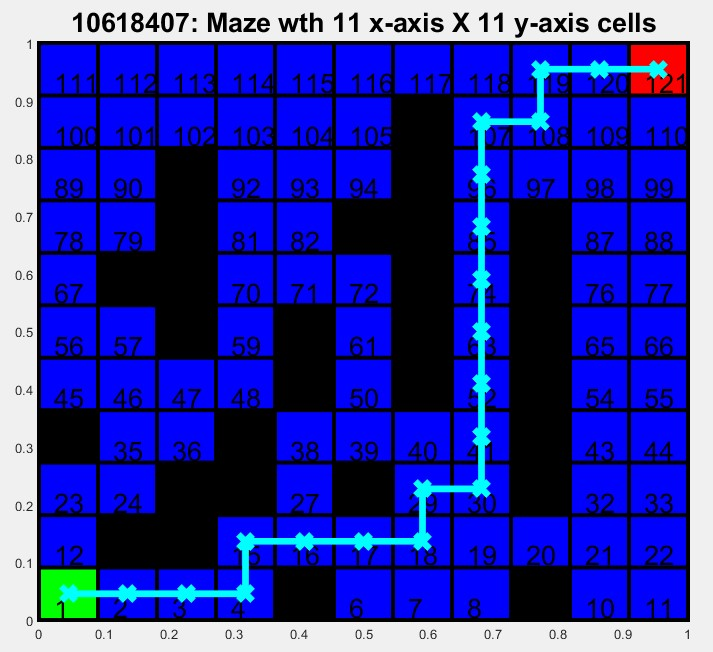
\includegraphics[width=9cm]{maze_solution_2}}
\caption{Plot of maze with path from highest Q-Values - solution 2}
\label{fig:maze_solution_2}
\end{figure}

\begin{figure}[H]
\centerline{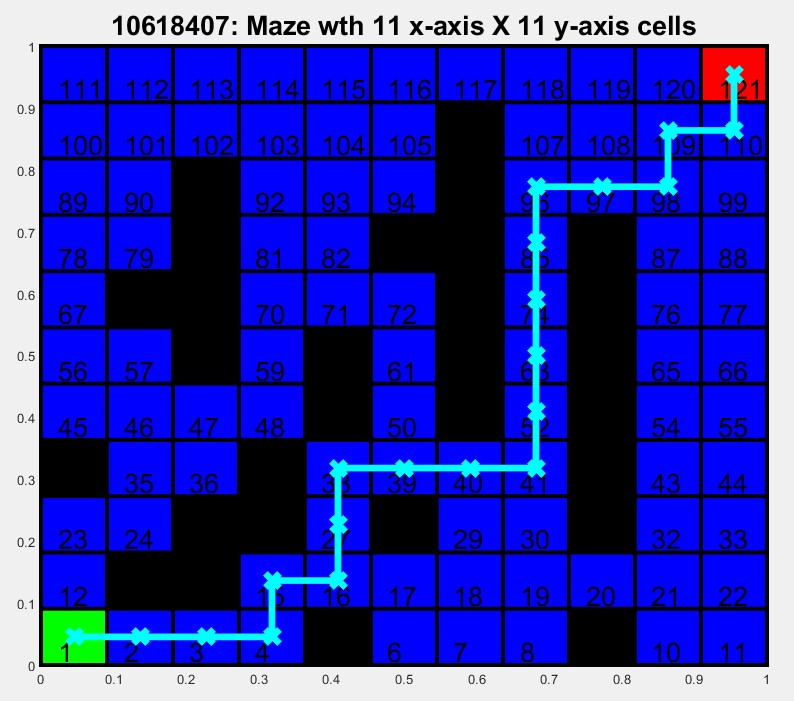
\includegraphics[width=9cm]{maze_solution_3}}
\caption{Plot of maze with path from highest Q-Values - solution 3}
\label{fig:maze_solution_3}
\end{figure}

It can be seen from figure~\ref{fig:maze_solution_1}, figure~\ref{fig:maze_solution_2}, and figure~\ref{fig:maze_solution_3} that there are multiple solutions to solving this maze in the shortest number of steps. The above figures are merely demonstrations of three of these possible solutions. 

\section{Move arm endpoint through maze}
\subsection{Generate kinematic control to revolute arm}

\begin{figure}[H]
\centerline{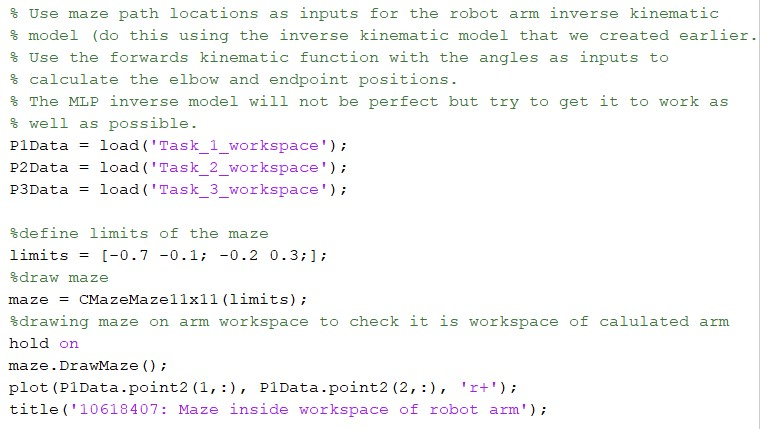
\includegraphics[width=10cm]{maze_inside_robot_workspace_code}}
\caption{Setting up maze limits and plotting it in the workspace of the arm}
\label{fig:maze_inside_workspace}
\end{figure}

\begin{figure}[H]
\centerline{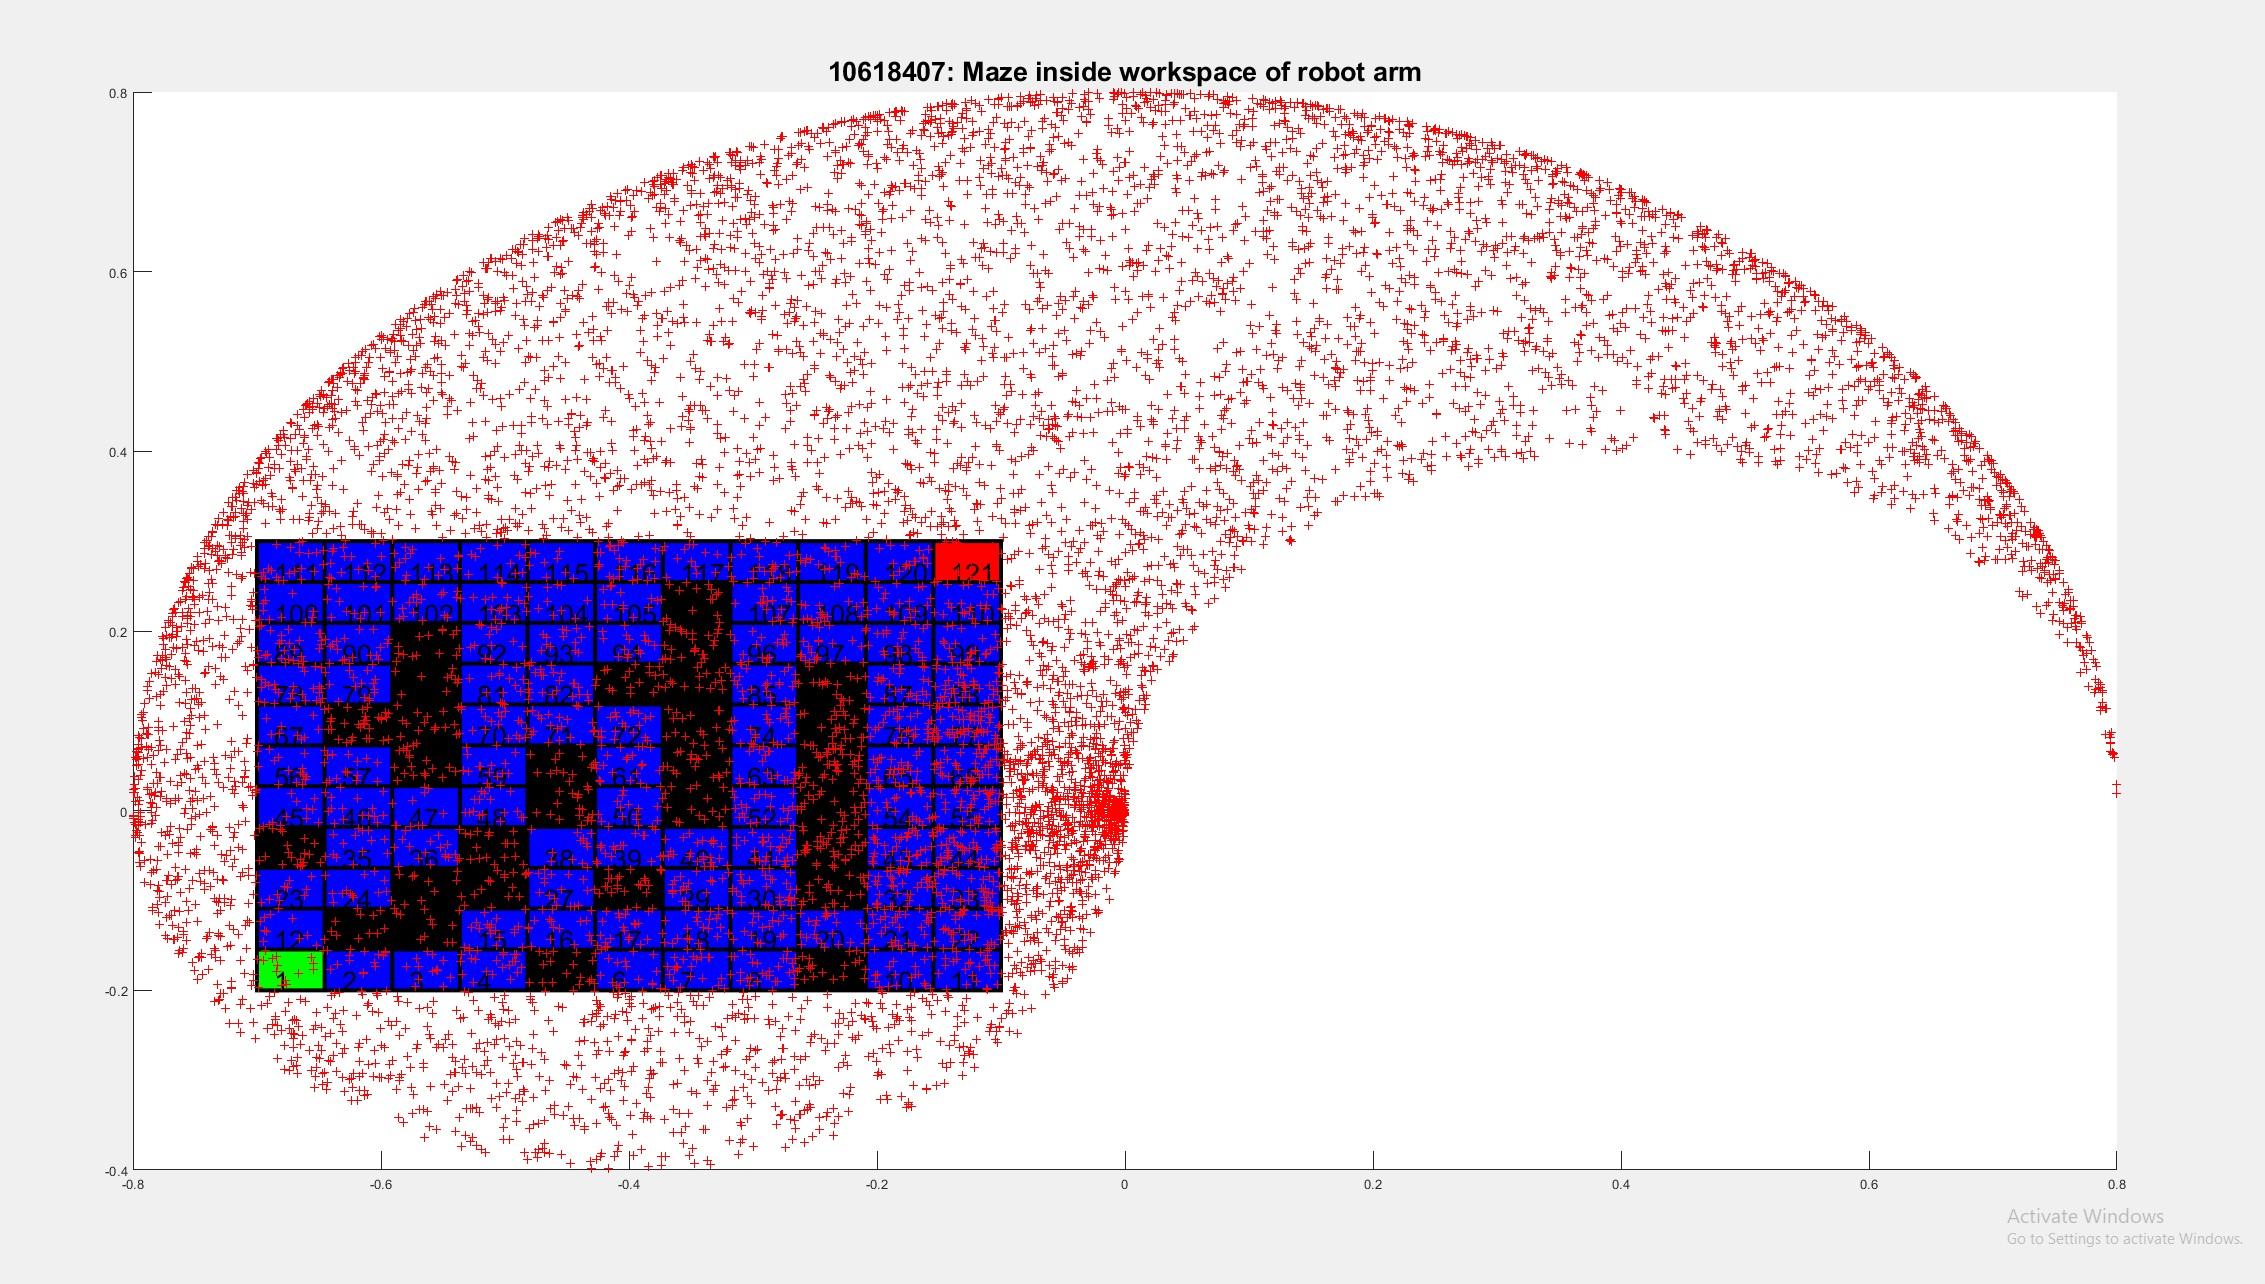
\includegraphics[width=15cm]{maze_inside_robot_workspace}}
\caption{Plot of robot arm workspace encompassing the maze}
\label{fig:maze_inside_workspace_plot}
\end{figure}

Figure~\ref{fig:maze_inside_workspace} and figure~\ref{fig:maze_inside_workspace_plot} show the scaling of the maze is correct. This is shown by the maze falling within the workspace of the robot arm. This means that the arm will be able to reach all locations in the maze.

\begin{figure}[H]
\centerline{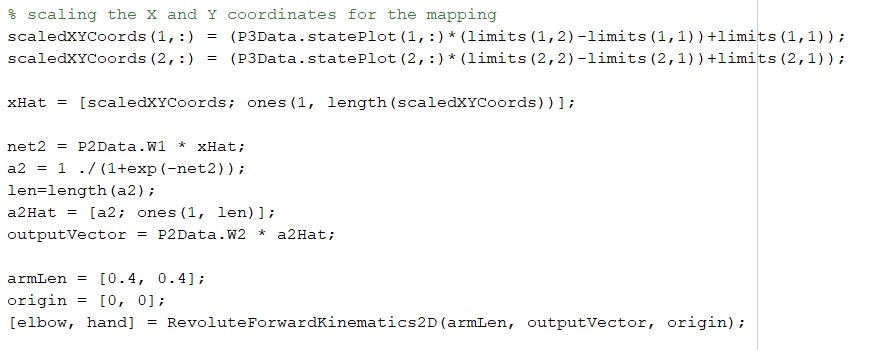
\includegraphics[width=15cm]{saled_feed_forward_pass_of_arm}}
\caption{Calculating the path's joint angles using a forward pass of the trained neural network}
\label{fig:feed_forward_pass_coords}
\end{figure}

Once the locations for the path are scaled, these new coordinates are passed into a feed forward pass of the neural network to calculate the joint angles. After the joint angles are calculated, these are then transformed into the positions of the end effector and joint via the 'RevoluteForwardKinematics2D' function. This generates  the points to be plotted onto the graph. 

\begin{figure}[H]
\centerline{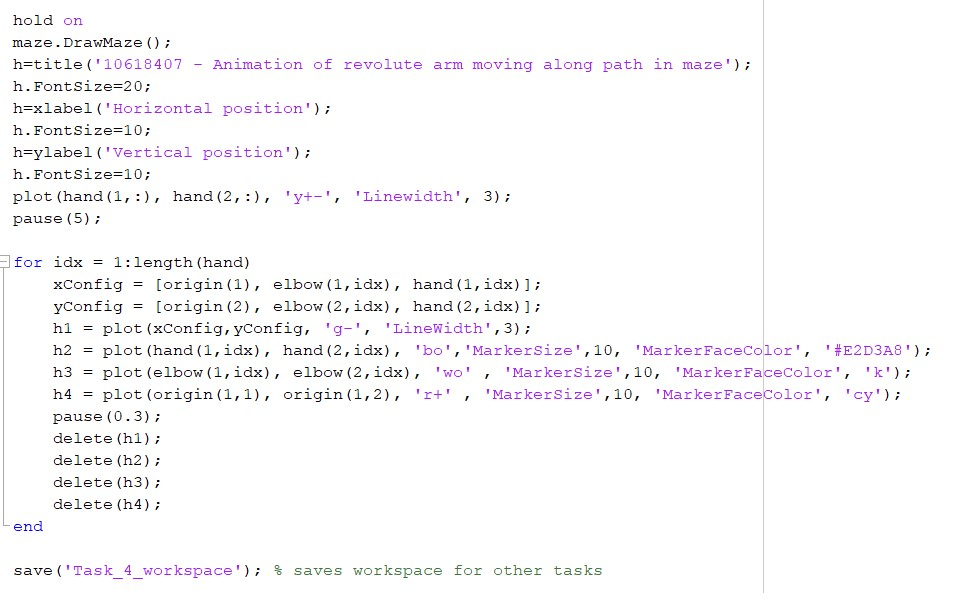
\includegraphics[width=15cm]{output_frames_on_maze}}
\caption{Calculating the path's joint angles using a forward pass of the trained neural network}
\label{fig:path_joint_code}
\end{figure}

\begin{figure}[H]
\centerline{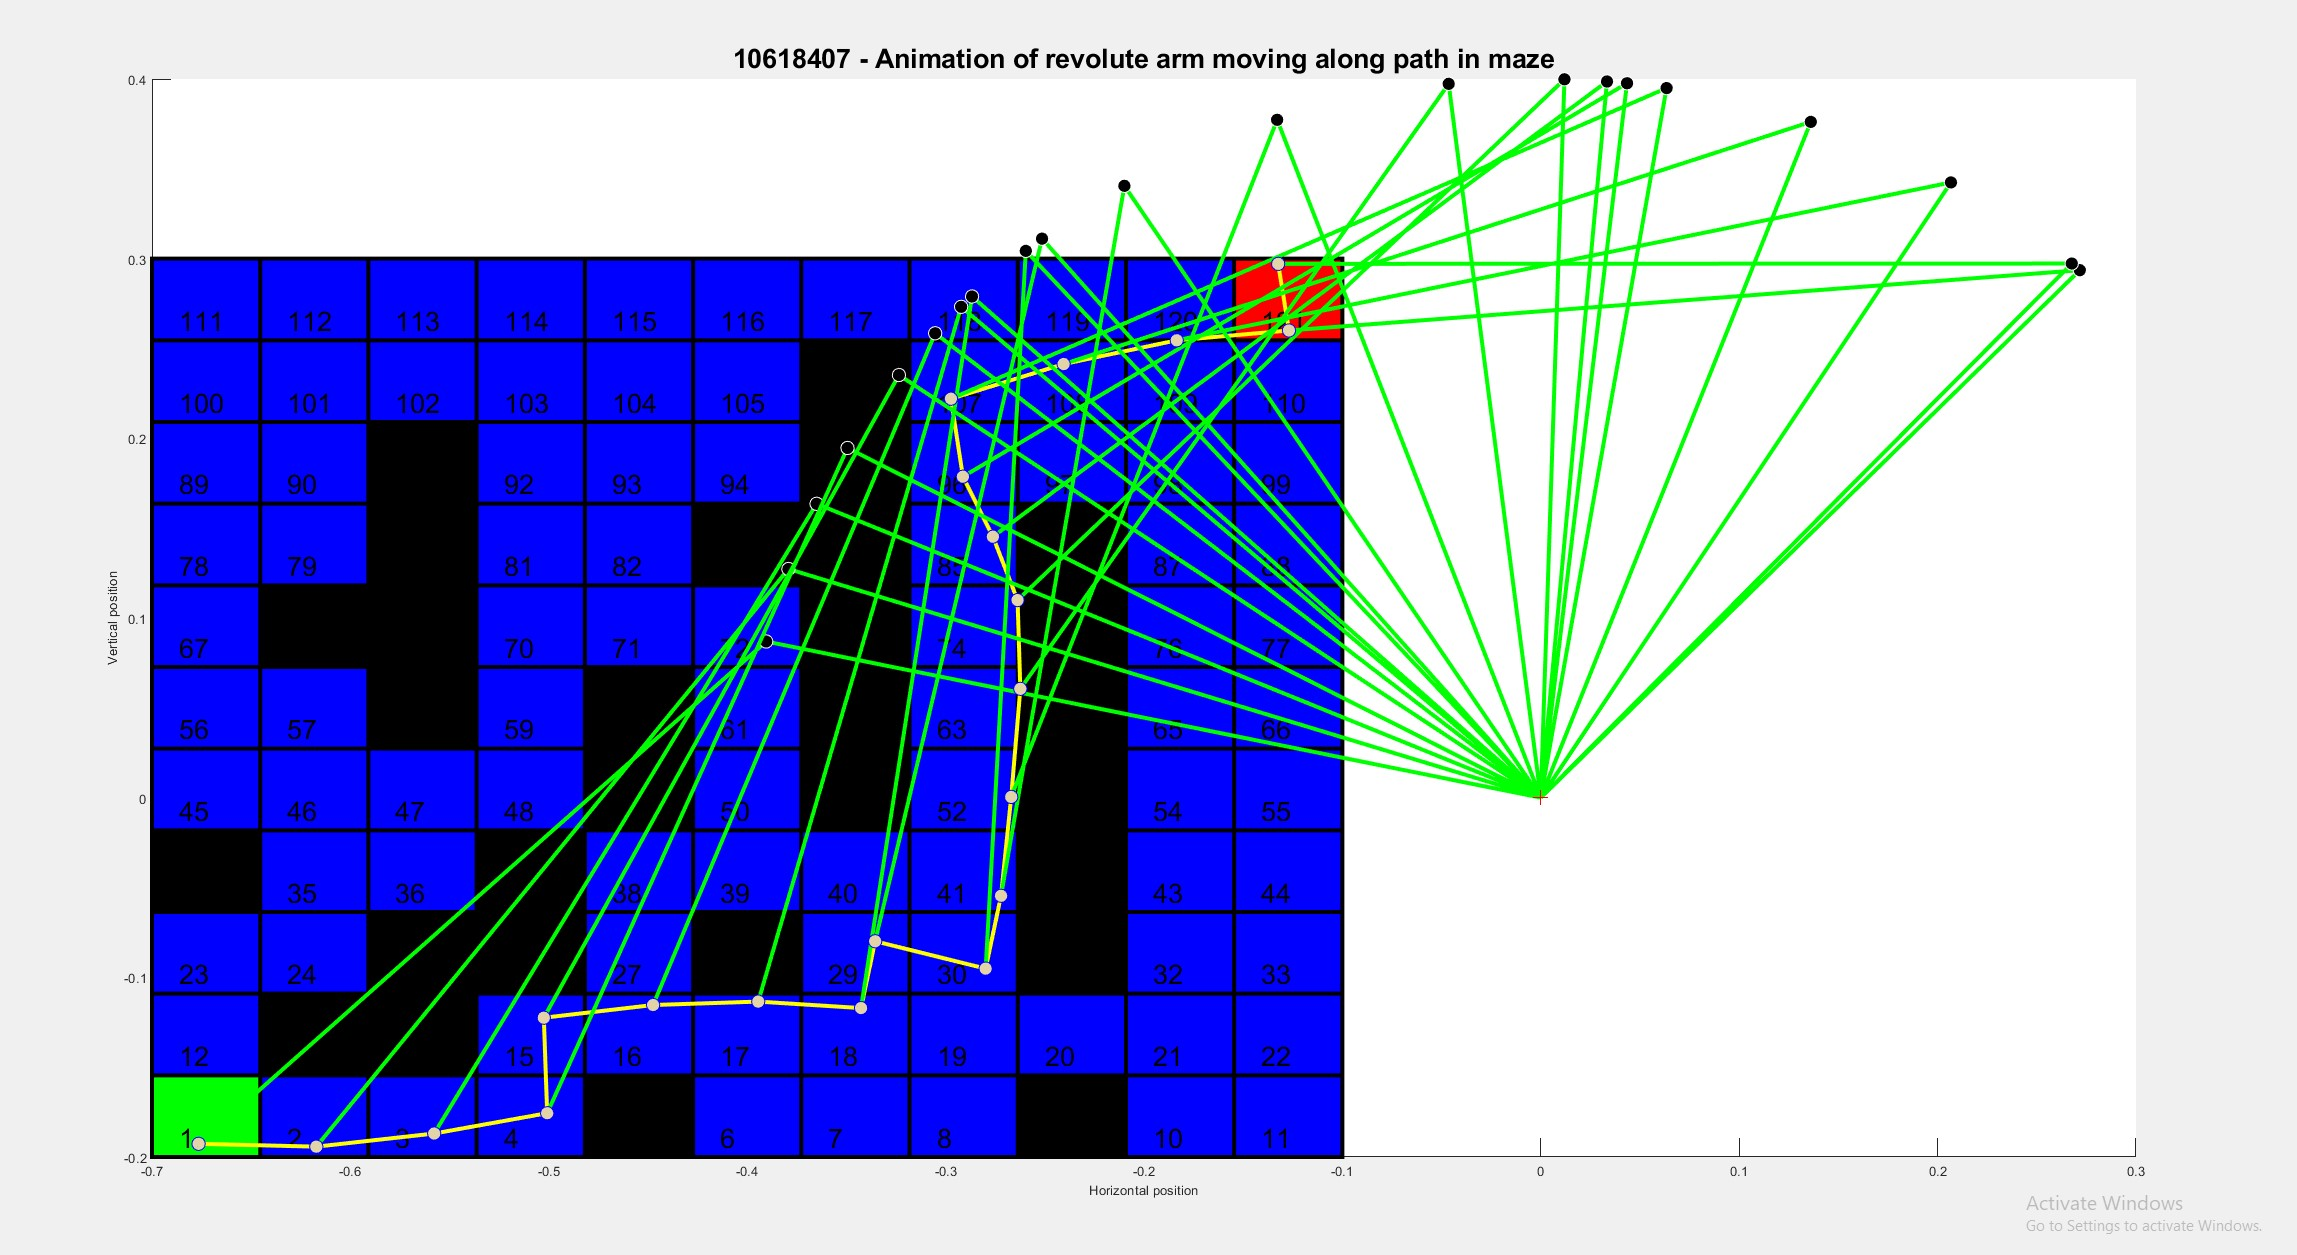
\includegraphics[width=15cm]{arm_moving-through_workspace}}
\caption{Superimposed Arm locations for each step on the maze}
\label{fig:arm_locations_on_maze}
\end{figure}

Figure~\ref{fig:arm_locations_on_maze} and figure~\ref{fig:path_joint_code} above show the path travelled by the arm. The plot code takes the locations calculated by the code in figure~\ref{fig:feed_forward_pass_coords} and plots them onto the maze workspace. The code iterates through the various locations and outputs them onto the maze. After this, the arm is deleted so the next one can be shown. This can be seen in the video linked below. Before the main iterative loop, the yellow line is plotted onto the maze. This line shows the path that the arm is taking through the maze. It can be seen that the plotted line falls within the correct states on the maze. This shows that the Q-Learning and Inverse Kinematic model have both produced their expected outputs, and have worked as intended. 

\subsection{Animate revolute arm movement} 

The animation of the arm moving through the maze can be seen here: - \href{https://youtu.be/_ZtAD1VYlzo}{Robot Arm Traversing Through The Maze}

\end{document}
